% SPDX-FileCopyrightText: Copyright (c) 2026 NVIDIA CORPORATION & AFFILIATES. All rights reserved.
% SPDX-License-Identifier: Apache-2.0
%
% ROLE: appendix D. The simulator, workload, calibration and freeze details behind sec:simulator
%   (and the warm-up rule of sec:objective) that a reader needs to audit or reproduce the setup but
%   not to follow the argument: policies in replay, engine facts, determinism across hosts, the
%   replicate protocol and its noise, replay cost; per-source workload details, AgentX recycling,
%   load-mode details and transforms; calibration rules, curves, windows and the session warm-up
%   fix; the freeze history. Moved here from simulator.tex and setup.tex at base <commit-50>.
% EVIDENCE: CR/config/engine.json; CR/facts/{setup,noise,noise_calibration,calibration,
%   agentx_lowered,test_freeze,remote,gate}.json; CR/facts/{DEVIATIONS,STATE}.md;
%   CR/traces/MANIFEST.json; CR/cells/SPLIT_MANIFEST.json; CR/runs/calibrate-fix-r0/{curves,decisions}.json;
%   CR/audits/{setup,calibration}/; WT/benchmarks/learned_routing/learned_routing/{replicates,cache,
%   cells}.py and workloads/{synthetic,transform,agentx_lowered}.py; plus the src comment on each block.

\section{Simulator, workload and calibration details}
\label{app:sim}

This appendix gives the details behind \cref{sec:simulator}, in the order of that section: the
replay environment, the workloads, the calibration and the freeze of the test set.

% ---------------------------------------------------------------------------------------------
\subsection{Replay}

\paragraph{Policies in replay.}
% src: CR/CONTRACT.md "Policy YAML"; WT/notes/learned-routing/campaign/PLAN.md "Starting point (verified)";
%      CR/facts/setup.json policy_selection_evidence (negative controls: unknown type and unknown
%      parameter are rejected naming the catalog); CR/facts/DEVIATIONS.md build B3 "canonical policy
%      files". Not claimed: that every malformed YAML errors (setup audit ais-and-policy r0 F2: a YAML
%      without worker_selection.aggregated silently ran the unseeded default).
Worker selection in replay goes through the same Rust policy catalog as in the live router, and a
policy is configured by the same policy YAML. Replay rejects unknown policy types and unknown
parameters by name, and the harness writes every policy YAML in one canonical form. Running catalog
policies inside offline replay is a feature of the branch this study builds on; on Dynamo's
main branch, replay rejects custom policies.

\paragraph{Engine facts.}
% src: CR/facts/setup.json ais_active_evidence.estimator_vs_replay_ttft_ms
%      (1024: estimator 55.4868010845058, replay 55.486801; 8192: 475.97461213209505 vs 475.974612)
A single 1,024-token request replayed alone has a TTFT of \SI{55.49}{ms}, equal to the \ais{}
estimator's prediction to within \SI{1}{ns}, and an 8,192-token request \SI{475.97}{ms}.
\Cref{tab:engine-ttft} compares \ais{} timing with the mock engine's built-in polynomial model. The
fallback model underestimates long prompts badly (7.2 times at 120,000 tokens), so a replay
without \ais{} would mislead about exactly the long-context traffic this study cares about.
% src: CR/facts/setup.json single_request_ttft_ms_ais_vs_polynomial (120000: 17815.54 vs 2476.95;
%      ratio computed here: 7.19)

% src: CR/facts/setup.json (long_context, single_request_ttft_ms_ais_vs_polynomial, ais_active_evidence)
\begin{table}[tbp]
  \centering\small
  \caption{Time to first token of one request replayed alone on an idle worker, with \ais{} timing
    and with the mock engine's built-in polynomial model, which replay falls back to when the
    bindings lack \ais{} support. Every replay in this paper uses \ais{} timing.}
  \label{tab:engine-ttft}
  \begin{tabular}{@{}lrrrrr@{}}
    \toprule
    Prompt length (tokens) & \num{1024} & \num{8192} & \num{32768} & \num{65536} & \num{120000} \\
    \midrule
    TTFT, \ais{} (ms) & 55.49 & 475.97 & \num{2550.45} & \num{6838.33} & \num{17815.54} \\
    TTFT, polynomial fallback (ms) & 32.49 & 169.14 & 676.55 & \num{1353.10} & \num{2476.95} \\
    \bottomrule
  \end{tabular}
\end{table}

% src: CR/facts/setup.json ais_active_evidence.prefill_ms_per_1k_tokens.chunk8192_after_prefix_tokens
%      (0: 59.50; 114688: 249.59)
Prefill cost per token grows with the context already in the KV cache: an 8,192-token chunk costs
\SI{59.5}{ms} per thousand tokens with no prefix and \SI{249.6}{ms} per thousand after a
114,688-token prefix.
% src: CR/facts/setup.json ais_active_evidence.decode_step_ms_by_batch_and_context
%      (b1_ctx2048 15.144; b128_ctx2048 29.176; b32_ctx8192 27.318; b8_ctx32768 26.511)
A decode step takes \SI{15.1}{ms} for one 2,048-token sequence and 26.5--\SI{29.2}{ms} for about
262,000 tokens of context in the batch, whether they are 128 sequences of 2,048 tokens, 32 of 8,192
or 8 of 32,768.
% src: arithmetic on CR/config/engine.json kv_capacity: 131072 / 301808 = 0.434; 66313 / 301808 = 0.220
%      (AgentX mean prompt: tab:trace-stats)
One request at the 131,072-token context limit would occupy 43\% of a worker's KV cache, and the
mean AgentX prompt (66,313 tokens) 22\%, so four or five AgentX contexts fill a worker.
% src: CR/facts/setup.json long_context.notes (corrected by audit setup/determinism-cost-context r1 F2)
Replay rejects a request whose prompt reaches the context limit and silently truncates the output
of one whose prompt plus output exceeds it; the trace transforms therefore drop or clamp such
rows explicitly (\cref{sec:workloads}).

\paragraph{Determinism across hosts.}
% src: CR/facts/setup.json determinism (per_request_identical; request UUIDs only reorder the
%      output) and replay_cost.in_process_repeats
Within one process and across fresh processes a seeded replay reproduces every per-request row;
request UUIDs only reorder the output (\cref{app:determinism}).
% src: CR/CONTRACT.md A9 addendum and A10; CR/facts/remote.json parity.core_6_train_cells.remote_vs_fresh_local
%      (28/28 records identical, 186,548 per-request rows compared); the later node-image smoke with the
%      same counts is a separate entry in remote.json, described in app:parity
Bit-exact results also need the same operating-system image, because replay calls the host's
math library. Each distinct remote CPU node image (operating system and C library) was checked
against the workstation before use: on the first check, 28 of 28 remote records and all 186,548
per-request rows matched a fresh local run. A node image added later passed its own check with the
same counts (\cref{app:parity}).

\paragraph{Where noise comes from.}
% src: CR/facts/noise.json why, finding_verdict; CR/audits/setup/determinism-cost-context-r0.md
Because a replay is deterministic, running it twice measures nothing; the setup audit rejected
the original plan to estimate noise that way (\cref{tab:audits}). What is arbitrary in a recorded
workload is the order of requests logged at the same instant.
% src: CR/traces/MANIFEST.json mooncake stats (distinct_first_arrivals 1180, first_arrival_span_ms
%      3600000 -> 3,053 ms grid); WT/benchmarks/learned_routing/learned_routing/replicates.py docstring
%      ("3 s bursts of up to 47 rows"); CR/facts/calibration.json rules.replicates (3053 / 3000 / 1000 ms)
The Mooncake trace has 1,180 distinct timestamps in its hour, a grid of about \SI{3053}{ms}, and
up to 47 requests share one; the generated sessions use a \SI{1}{s} grid. Replay delivers each
burst at once and places it in file order.

\paragraph{The replicate protocol.}
% src: WT/benchmarks/learned_routing/learned_routing/replicates.py (PROTOCOL, SPREAD_PROTOCOL,
%      replicate_seed, policy_seed, permute_*, spread_mooncake_arrivals); CR/CONTRACT.md A1;
%      CR/facts/DEVIATIONS.md 2026-10-02 calibration "arrival spread replicates"
Replicate $\krep$ of a cell re-draws only that arbitrary part of the trace, and the same
replicate is used for every policy (common random numbers):
\begin{itemize}
  \item \textbf{Arrival spread} (\code{crn-spread-v1}; Mooncake, FAST25 conversation and
    sessions). Each session's first arrival moves to a uniform random point inside its logging
    slot (\SI{3053}{ms}, \SI{3000}{ms} and \SI{1000}{ms} for the three traces); sessions are
    re-sorted by the new times and later turns keep their completion-relative delays.
  \item \textbf{Order permutation} (\code{crn-order-v1}). FAST25 synthetic, whose timestamps are
    nearly unique, permutes the sessions that tie; AgentX permutes the order of its recycled
    play copies, which re-deals them to lanes (\cref{sec:agentx}).
  \item \textbf{Policy seed} $\krep + 1$ for every policy that takes a seed.
\end{itemize}
The replicate seed is a hash of the protocol, the source trace's SHA-256 and $\krep$. Cells that
share a trace (other $\Nw$, other load level) therefore share their replicates, and every
replicate, including $\krep = 0$, is a fresh draw, so the recorded file order has no special
status.
Spreading arrivals is also a modeling choice, discussed in \cref{sec:replicates}.

\paragraph{Replicate noise.}
% src: CR/facts/noise.json measured_setup_fix_r0 (goodput_cv_by_policy, 8 replicates, three
%      uncalibrated 2,000-request Mooncake cells: min 0.01169 rr n4-open, max 0.0385 lmetric n4-open);
%      CR/facts/noise_calibration.json pooled_paired_ratio_sd_by_family_N_mode (min 0.00365
%      sessions N32 open, max 0.0448 sessions N2 open)
Replicates move goodput by amounts comparable to the effects of interest. On three uncalibrated
2,000-request Mooncake cells, goodput varied across 8 replicates with a coefficient of variation
of 1.2--3.9\% for every policy tested. On the calibrated cells, the standard deviation of
round robin's per-replicate goodput ratio against $\piref$, pooled by family, $\Nw$ and load
mode, ranges from 0.004 to 0.045. Segment heterogeneity, not replicate noise, limits what the
study can resolve (\cref{sec:noise-floor}).

\paragraph{Cost.}
% src: CR/facts/setup.json replay_cost (fresh process 1.43-1.67 s for 2,000 requests at N = 2..32);
%      CR/audits/setup/determinism-cost-context-r0.md (full trace 7.64 s at N = 8, 8.77 s at N = 32);
%      CR/facts/agentx_lowered.json caveats [8] (2.9-4.9 ms per row; N = 32 lanes cells 2-4 min);
%      WT/benchmarks/learned_routing/learned_routing/cache.py (key fields)
A 2,000-request Mooncake replay takes about \SI{1.5}{s} of one CPU core in a fresh process, nearly
flat in $\Nw$ from 2 to 32, and the full 23,608-request trace 7.6--\SI{8.8}{s}. AgentX traffic
costs 2.9--\SI{4.9}{ms} per request, so an AgentX cell at $\Nw = 32$ takes 2--4 minutes. Results
are cached under a key built from the policy, the cell's content, the replicate, the harness
version and the replay build, so a rebuilt binding or an edited cell can never return a stale
result (\cref{app:determinism}).

% ---------------------------------------------------------------------------------------------
\subsection{Workloads}
\label{app:workloads}

\paragraph{Mooncake slices.}
% src: CR/facts/DEVIATIONS.md 2026-10-02 build fixer r0 (audit S1)
An earlier design used overlapping 12-minute Mooncake slices, in which each window's warm-up was
the previous window's measurement; an audit found that half of test window w3's scored rows were
also replayed in train cells, and the slices were redesigned before calibration. No row now
appears in two slices.
% src: CR/facts/STATE.md fix(build r0) ("hygiene 0 shared rows across all segment pairs");
%      CR/facts/STATE.md audit(build/harness-robustness-splits r0) (1,634/3,245 = 50.4%)

\paragraph{FAST25.}
% src: CR/traces/MANIFEST.json roles and stats (fast25_conversation: 91% skeleton, reuse 0.384 vs
%      0.630, 1 root; fast25_synthetic: independent, near-unique timestamps, max ISL 191,378);
%      CR/facts/DEVIATIONS.md 2026-10-02 build fixer r0 (FAST25 synthetic windows [0, 8.5) and [8.5, 17) min)
The FAST25 conversation trace shares Mooncake's (timestamp, prompt length, output length) skeleton
on 91\% of rows but has a different prefix structure (reuse 0.38 against 0.63, one shared first
block). The synthetic trace has nearly unique timestamps; it is cut into two windows of 8.5
minutes, each with a 3-minute warm-up.

\paragraph{The excluded tool-agent trace.}
% src: CR/traces/MANIFEST.json toolagent role ("identical OSL on 23,608/23,608 rows, 0-conflict hash
%      bijection over 409,356 aligned blocks, reuse correlation 0.9998, timestamps x0.9825");
%      CR/audits/setup/determinism-cost-context-r1.md F1
A further trace from that release, the tool-agent trace, is excluded from every split.
It is a relabeled copy of the Mooncake trace: its output lengths match on all 23,608 rows, its
hash blocks map one-to-one onto Mooncake's over 409,356 aligned blocks with no conflict, and its
timestamps are Mooncake's scaled by 0.9825. Including it would have put the same workload in two
families, and possibly in two splits.

\paragraph{The session generator.}
% src: WT/benchmarks/learned_routing/learned_routing/workloads/synthetic.py (module docstring,
%      SessionSpec defaults); CR/traces/MANIFEST.json provenance.spec of sessions_seed{0..9};
%      CR/facts/DEVIATIONS.md 2026-10-02 build B2 "synthetic sessions are a generated Mooncake session trace"
In replay's built-in synthetic-session source every request has the same prompt and output length,
every inter-turn delay is the same constant, and a later turn does not extend the earlier turns'
context. The study's generator writes its sessions as a Mooncake session trace. Sessions start
as a Poisson process at one per second, floored to a \SI{1}{s} grid. Each draws one of 16 system
prompts with Zipf popularity (exponent 1.1; lognormal length, median 2,000 tokens). Turns per
session are geometric with mean 5 (at most 24); user messages are lognormal (median 600 tokens for
the first, 250 later) and outputs lognormal (median 250, at most 2,000), and a session ends before
its context would exceed 49,152 tokens. Each later turn is released an exponential think time
(mean \SI{8}{s}) after the previous turn completes.
% src: CR/traces/MANIFEST.json synthetic_sessions/long/* provenance.lengthening ("same generator seed
%      with a longer duration_s; the generator is sequential, so the original 720 s trace is a byte
%      prefix"; duration_s 48000)
For the calibrated cells each seed was regenerated with a \SI{48000}{s} duration; the generator is
sequential, so the \SI{720}{s} trace is a byte prefix of the long one, which adds independent
sessions from the same seed rather than copies.

\paragraph{AgentX source.}
% src: CR/traces/MANIFEST.json agentx (source: semianalysisai/cc-traces-weka-062126 @ 23f152f6,
%      393 plays, 98,827 requests; selection: predicate, 82 plays, 3,132 requests); moved from
%      simulator.tex in restructure round 1 (E2)
The AgentX plays are the public dataset \file{semianalysisai/cc-traces-weka-062126} at revision
\code{23f152f6} \citep{agentxtraces}, 393 plays and 98,827 requests, of which the context rule of
\cref{sec:workloads} keeps 82 plays and 3,132 requests.

\paragraph{AgentX idle gaps.}
% src: CR/facts/DEVIATIONS.md 2026-10-02 build B2 "every AgentX derived trace caps idle gaps at 300 s"
%      (140 of 2,666 gaps in 56 of 82 plays exceed 300 s, up to 355,532 s; 399,658 s uncapped vs
%      11,942 s capped)
Recorded gaps include users stepping away for hours: 140 of 2,666 gaps (in 56 of 82 plays)
exceed \SI{300}{s}, the longest \SI{355532}{s}. Every AgentX trace caps idle gaps at
\SI{300}{s} with a monotone time warp that keeps every busy period, request duration and
ordering; uncapped, the 82 plays would simulate for \SI{399658}{s} instead of \SI{11942}{s},
mostly idle.

\subsubsection{Recycling AgentX plays at any worker count}
\label{sec:agentx}\label{app:agentx}

% src: CR/CONTRACT.md A3 ("Why"); WT/benchmarks/learned_routing/learned_routing/workloads/agentx_lowered.py
%      module docstring; CR/facts/DEVIATIONS.md 2026-10-02 build B2 (no N = 16/32 cells)
Replaying the plays natively cannot hold a steady AgentX load on many workers. In timestamp mode
every play's root starts at time zero; in lanes mode the plays are dealt to lanes once and never
reused, so 82 plays cannot keep 16 or 32 workers busy, and the first design had no AgentX cell
above $\Nw = 8$. We therefore convert each play once into \aisim{}'s Agentic Mooncake v2 trace
format and recycle copies of it.
% prov: A3
\begin{itemize}
  \item \textbf{Lowering.} The conversion is \aisim{}'s own: a small Rust tool calls the public
    Weka importer of the \code{aisimulate-core} version the bindings link, so the rows are the
    importer's output, not a reimplementation.
    % src: CR/facts/agentx_lowered.json method.summary ("81-line Rust CLI ... WekaImporter")
  \item \textbf{Copy isolation.} Each copy of a play gets fresh play, session and request
    identifiers and its own consecutive range of hash identifiers. Replay interns hash
    identifiers globally across a file, so without the new range two copies of one play would
    share KV prefixes; with it, copies never do. Dependency edges, delays and lengths are copied
    unchanged.
  \item \textbf{Draws.} Each cell draws its copies with replacement from its own segment's plays,
    so segments remain independent workloads.
    % src: CR/facts/DEVIATIONS.md 2026-10-02 calibration "AgentX cells use the A3 lowered traces with
    %      per-segment play subsets"; one train cell pools A1 and A2 (agentx-A1_A2-base-n8-lanes-L3)
  \item \textbf{Lanes.} Every AgentX cell runs closed: a fixed number of lanes per worker, each
    lane running its dealt copies back to back, with many more copies than lanes so that every
    lane stays busy through the measurement window. The lowering also supports open-loop Poisson
    play arrivals, but open-loop AgentX has a cliff between 0.002 and 0.0025 plays per second per
    worker, past which the number of plays in flight keeps growing; no stationary
    open-loop load reaches the L3 band, so no cell uses it.
    % src: CR/facts/agentx_lowered.json suggested_loads.open_mode.cliff ("between 0.002 and 0.0025 plays/s
    %      per worker the open system loses its steady state at every N ... The A2 L3 target (0.65)
    %      therefore has no stationary open-loop load")
\end{itemize}
% src: CR/facts/agentx_lowered.json parity_evidence.graph_digests (82/82 per transform, six transforms)
%      and parity_evidence.replay (exact_cases 84, exact_identical 84; plays, workers [2, 4], policies;
%      tiers single/corpus/recycle) and per_transform (84/84 each)
The conversion preserves replay semantics exactly where it can be compared with native replay.
For all 82 plays and each of the six play transforms the cells use, the native graph and the
converted file compile to the same canonical graph digest. Replaying six plays that cover
subagents, joins and concurrent spawns (alone, as one corpus, and as a 12-copy recycled corpus,
at $\Nw = 2$ and 4, under the seeded default and round robin) gave identical per-request records
in 84 of 84 cases for every transform.
% src: CR/facts/agentx_lowered.json parity_evidence.node_order_sensitivity (12/12 differ; mean e2e
%      -7.4% to +4.7%); caveats [0], [12] (osl 1.5: -5.7..+18.0%; osl 2.5: -15.6..+13.5%; N = 2)
The order of copies within a file is a free choice: the same recycled corpus in a different copy
order changed mean end-to-end latency by $-7.4\%$ to $+4.7\%$ for the untransformed plays, and by
up to $-15.6\%$ and $+18.0\%$ under the output-length transforms, in a synchronized-start worst
case at $\Nw = 2$.
That is the same kind of variation as a replicate, and the replicate protocol re-draws it
(\cref{sec:replicates}).

\subsubsection{Load-mode details}

% src: CR/facts/DEVIATIONS.md 2026-10-02 calibration "think-time-invariant sessions" (8 s mean think at
%      N = 2 vs about 0.3 s at N = 32; 540 s windows shrank to about 19 s of replay at N = 32)
Replay's speedup divides inter-turn delays as well as arrival times. In the first session cells
this meant that think time shrank with load and with $\Nw$: at matched per-worker load the mean
think time was \SI{8}{s} at $\Nw = 2$ and about \SI{0.3}{s} at $\Nw = 32$. Session cells now
pre-multiply each delay by the speedup, so a user's think time is the same at every load and
every $\Nw$; only the session arrival rate scales. Release is causal in both multi-turn
families: a session's next turn waits for the previous turn to complete, and an AgentX request for
the requests it depends on \citep{rajib2026agentservesim}. Open-loop arrivals of flat traces do not
react to latency, a known bias of trace-driven evaluation \citep{alomar2023causalsim}.
% src: CR/literature/LESSONS.md LR-09 (Schroeder principle (vii): >= 10 requests per session; AgentX
%      3,132/82 = 38.2 requests per play); causal release: LR-09 [code] aisimulate-core
%      replay/loadgen/driver.rs:3320; CR/facts/agentx_lowered.json caveats [3]
AgentX plays average 38 requests each, well past the point at which a partly-open system behaves
as a closed one \citep{schroeder2006open}, which is one more reason lanes are its natural mode.

\subsubsection{Transforms}

% src: WT/benchmarks/learned_routing/learned_routing/workloads/transform.py (module docstring, order 1-7);
%      CR/cells/SPLIT_MANIFEST.json train_ranges and transform_tags; CR/cells/test.jsonl transform cells
Transforms vary the workload along axes a deployment might drift on, so that the test set can ask
whether a policy extrapolates. They are deterministic and seeded, applied in a fixed order, and
each derived trace is stored under the SHA-256 of its bytes with a record of its specification,
sources and realized statistics.
\begin{itemize}
  \item \textbf{Prompt length, shared and unique parts separately.} A block that occurs in two or
    more requests is \emph{shared}; it is expanded by the same seeded per-hash draw wherever it
    occurs, so hash identity stays consistent. Each request's \emph{unique} suffix is scaled
    on its own.
  \item \textbf{Output length.} Each $\OSL$ is multiplied, rounded and kept at least 1.
  \item \textbf{Prefix roots.} The shared root segment of the requests that start with the same
    block (a system prompt) is split into several disjoint hash-space copies (two to four here),
    and each request family below it goes to one copy; sharing within a family is unchanged, but
    there are proportionally more distinct system prompts.
  \item \textbf{Think time.} Session delays are scaled; AgentX plays are dilated in time about
    their first request, which scales every recorded gap and keeps every ordering.
  \item \textbf{Context cap.} Rows whose prompt reaches 131,072 tokens are dropped and outputs
    are clamped so that prompt plus output fits (AgentX plays, which cannot lose a request
    without breaking their graph, clamp outputs only).
\end{itemize}

% ---------------------------------------------------------------------------------------------
\subsection{Calibration}
\label{app:calibration}

\paragraph{Load levels.}
% src: CR/facts/calibration.json rules.levels[0..3]; WT/notes/learned-routing/REPRODUCE.md step 10
%      (interp_level: linear in log(load) between the bracketing grid points, 6 significant digits)
Each level is interpolated linearly in log-load between the two grid points that bracket it.
% src: CR/facts/calibration.json step4_reference.per_cell (48 train/val cells, default
%      good_frac_window_mean: min 0.4229 sessions-s1-base-n4-open-L3, max 0.9648
%      mooncake-w4-base-n8-open-L1); CR/audits/calibration/independent-rerun-r1.md minor F4 (wide
%      realized bands)
The bands are targets for the mean over train segments, not for each cell: on individual train
and validation cells, $\piref$'s realized good fraction ranges from 0.423 to 0.965.

\paragraph{The knee and the SLO fixed point.}
% src: CR/facts/calibration.json rules.sla[0..5], sla.<family> (anchor_mode, fixed_point_history,
%      knee_fraction 0.9); CR/facts/DEVIATIONS.md 2026-10-02 calibration "SLA rule (A2 form, knee-anchored)"
The SLO of \cref{eq:good} has two bounds per family, set at $\Nw = 8$ in the family's primary
mode:
\begin{itemize}
  \item the \emph{knee} marks where $\piref$ starts to saturate: in open loop, it is the load at
    which the mean slowdown of the last third of in-window arrivals exceeds the first third's by
    more than 15\%; in lanes, the load at which completions per second reach 0.95 of the grid's
    maximum (sessions use a different rule, below);
  \item $\Smax$ is chosen so that $\piref$'s good fraction is 0.65 at 0.9 times the knee, which
    makes that load L3;
  \item $\Imax$ is 1.2 times the 95th percentile of $\piref$'s per-request mean ITL at L2.
\end{itemize}
L2 depends on $(\Imax,\Smax)$ and $\Imax$ depends on L2, so the three are iterated to a fixed
point; for Mooncake, $\Imax$ went from 260.31 to 253.78 to \SI{252.12}{ms}.
% src: CR/facts/calibration.json sla.mooncake.fixed_point_history (itl 260.30981764, 253.77791533,
%      252.11716249)

\paragraph{Headroom below the knee.}
% src: CR/facts/DEVIATIONS.md 2026-10-02 calibration "SLA rule" (S = 5.69 for Mooncake; train cells
%      mooncake-w0-base-n4-open-L3 0.243 with CV 0.33, mooncake-w0-islu1.5-n4-open-L2 0.018;
%      after 10% headroom 0.548 and 0.817; runs/calibrate/step4_r1, step4_r4)
The 10\% headroom below the knee matters. A first version anchored L3 at the knee itself, which
gave Mooncake $\Smax = 5.69$ and left two train cells near the open-loop cliff with good
fractions of 0.243 and 0.018; with the headroom they are 0.548 and 0.817.

\paragraph{Load curves.}
% src: CR/runs/calibrate-fix-r0/curves.json (N = 8; RR at the levels: gf_rr_interp); points as plotted
\Cref{fig:load-curves} shows what the levels mean. In the primary modes the bands are steep: on
sessions, $\piref$'s good fraction falls from 0.95 to 0.65 between 0.350 and 0.409 sessions per
second per worker, and round robin, which ignores where a conversation's history is cached, is
already at 0.198 at L2. On Mooncake's closed loop the two curves stay within 0.04 of each other
up to L3 and cross just below it.

% Colors of the calibration figure (validated with the dataviz palette checker: blue/orange pass
% lightness, chroma, CVD and contrast checks on a light surface). Round robin is also dashed, so
% the figure stays readable in grayscale.
\definecolor{simPi}{HTML}{2A78D6}
\definecolor{simRR}{HTML}{EB6834}
\pgfplotsset{
  simcurve/.style={
    width=\linewidth, height=0.9\linewidth,
    ymin=0, ymax=1.03, ytick={0,0.5,1},
    extra y ticks={0.65,0.85,0.95}, extra y tick labels={},
    extra y tick style={grid=major, major grid style={densely dotted, black!45}},
    tick label style={font=\scriptsize}, label style={font=\scriptsize},
    title style={font=\footnotesize, yshift=-3pt},
    axis line style={black!60}, tick style={black!60},
    legend style={font=\scriptsize, draw=none, fill=none},
    every axis plot/.append style={line width=0.9pt, mark size=1.3pt},
  },
  simpi/.style={color=simPi, solid, mark=*},
  simrr/.style={color=simRR, densely dashed, mark=square*, mark options={solid}},
}
% Vertical lines at the calibrated L1, L2, L3 of one panel.
\newcommand{\simLevelLines}[3]{%
  \draw[black!35, thin] (axis cs:#1,0) -- (axis cs:#1,1.03);
  \draw[black!35, thin] (axis cs:#2,0) -- (axis cs:#2,1.03);
  \draw[black!35, thin] (axis cs:#3,0) -- (axis cs:#3,1.03);}

% Data: CR/runs/calibrate-fix-r0/curves.json, by_n["8"].curve[*] (load, gf_default, gf_rr), mirrored at
% WT/notes/learned-routing/campaign/runs/calibrate-fix-r0/curves.json; levels from
% CR/runs/calibrate-fix-r0/decisions.json levels.<family>.<mode>["8"]. gf values rounded to 3 decimals;
% Mooncake open-loop loads divided by 1,000. Replicates per point: 6 (Mooncake, AgentX), 8 (sessions).
\begin{figure}[tbp]
  \centering
  \begin{minipage}[t]{0.325\linewidth}
    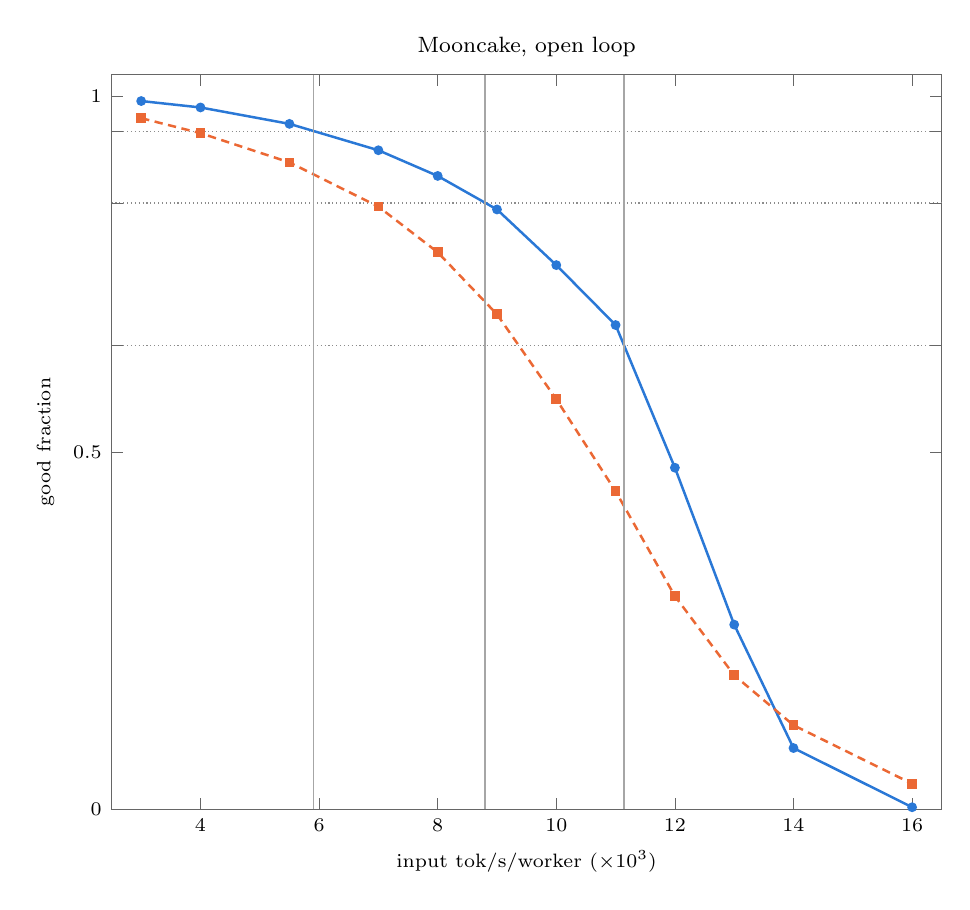
\begin{tikzpicture}
      \begin{axis}[simcurve, title={Mooncake, open loop},
          xlabel={input tok/s/worker ($\times 10^3$)}, ylabel={good fraction},
          xmin=2.5, xmax=16.5,
          % The legend is typeset in the empty sixth slot, where it covers no marker.
          legend to name=simloadlegend, legend cell align=left]
        \addplot[simpi] coordinates {(3,0.993) (4,0.984) (5.5,0.961) (7,0.924) (8,0.888)
          (9,0.841) (10,0.763) (11,0.679) (12,0.479) (13,0.259) (14,0.086) (16,0.003)};
        \addplot[simrr] coordinates {(3,0.969) (4,0.948) (5.5,0.907) (7,0.845) (8,0.781)
          (9,0.694) (10,0.575) (11,0.446) (12,0.299) (13,0.188) (14,0.118) (16,0.036)};
        \legend{$\piref$, round robin}
        \simLevelLines{5.90316}{8.79797}{11.1415}
      \end{axis}
    \end{tikzpicture}
  \end{minipage}\hfill
  \begin{minipage}[t]{0.325\linewidth}
    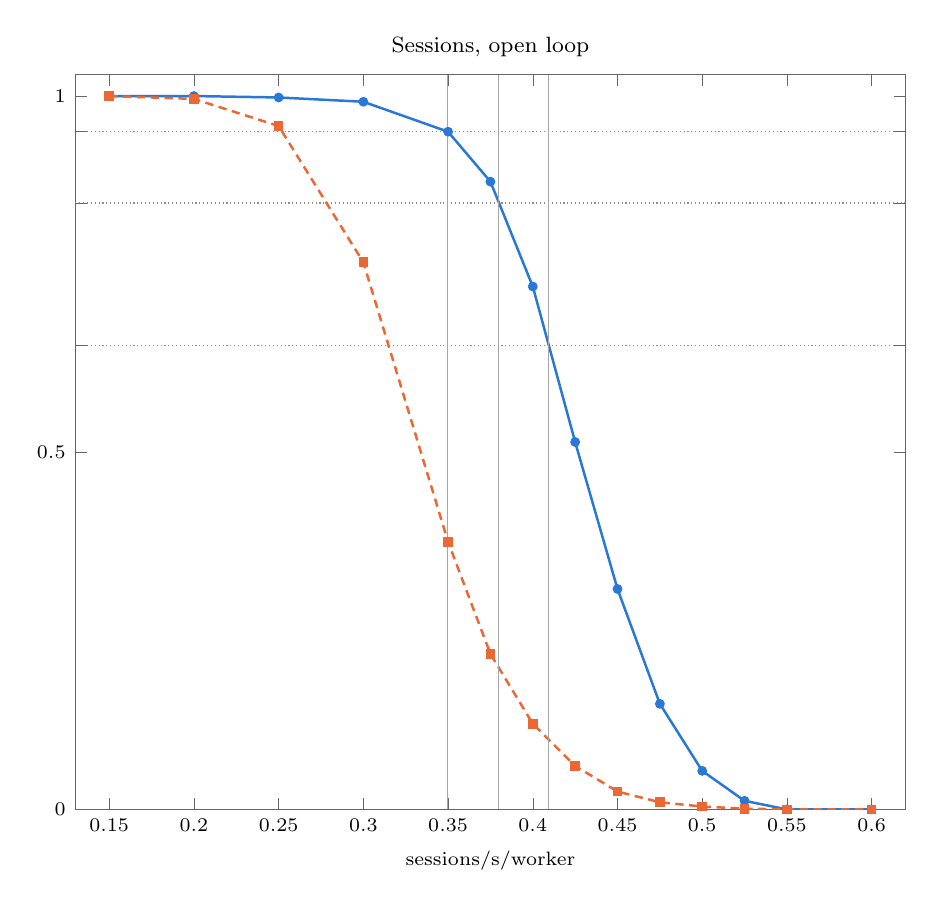
\begin{tikzpicture}
      \begin{axis}[simcurve, title={Sessions, open loop},
          xlabel={sessions/s/worker}, xmin=0.13, xmax=0.62]
        \addplot[simpi] coordinates {(0.15,1.000) (0.2,1.000) (0.25,0.998) (0.3,0.992)
          (0.35,0.950) (0.375,0.880) (0.4,0.733) (0.425,0.515) (0.45,0.309) (0.475,0.148)
          (0.5,0.054) (0.525,0.012) (0.55,0.000) (0.6,0.000)};
        \addplot[simrr] coordinates {(0.15,1.000) (0.2,0.996) (0.25,0.958) (0.3,0.767)
          (0.35,0.375) (0.375,0.218) (0.4,0.120) (0.425,0.061) (0.45,0.025) (0.475,0.010)
          (0.5,0.004) (0.525,0.001) (0.55,0.000) (0.6,0.000)};
        \simLevelLines{0.349709}{0.380012}{0.409343}
      \end{axis}
    \end{tikzpicture}
  \end{minipage}\hfill
  \begin{minipage}[t]{0.325\linewidth}
    \begin{tikzpicture}
      \begin{axis}[simcurve, title={AgentX, lanes},
          xlabel={lanes/worker}, xmin=1.8, xmax=7.2]
        \addplot[simpi] coordinates {(2,0.981) (2.5,0.959) (3,0.899) (4,0.783) (5,0.608)
          (6,0.403) (7,0.188)};
        \addplot[simrr] coordinates {(2,0.841) (2.5,0.746) (3,0.638) (4,0.483) (5,0.359)
          (6,0.287) (7,0.225)};
        \simLevelLines{2.57248}{3.38804}{4.73711}
      \end{axis}
    \end{tikzpicture}
  \end{minipage}

  \vspace{4pt}
  \begin{minipage}[t]{0.325\linewidth}
    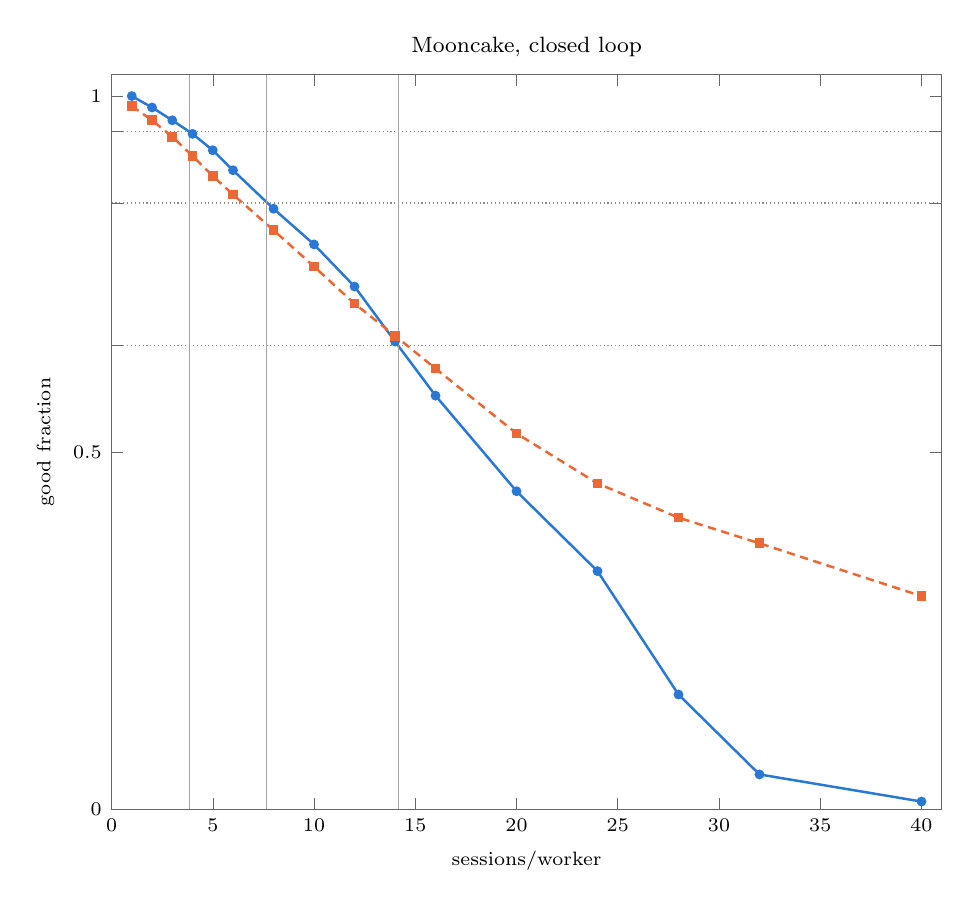
\begin{tikzpicture}
      \begin{axis}[simcurve, title={Mooncake, closed loop},
          xlabel={sessions/worker}, ylabel={good fraction}, xmin=0, xmax=41]
        \addplot[simpi] coordinates {(1,1.000) (2,0.984) (3,0.966) (4,0.947) (5,0.924)
          (6,0.896) (8,0.842) (10,0.792) (12,0.733) (14,0.656) (16,0.580) (20,0.446)
          (24,0.334) (28,0.161) (32,0.049) (40,0.011)};
        \addplot[simrr] coordinates {(1,0.986) (2,0.966) (3,0.943) (4,0.916) (5,0.888)
          (6,0.862) (8,0.812) (10,0.761) (12,0.709) (14,0.664) (16,0.618) (20,0.527)
          (24,0.457) (28,0.409) (32,0.373) (40,0.299)};
        \simLevelLines{3.84042}{7.67267}{14.1503}
      \end{axis}
    \end{tikzpicture}
  \end{minipage}\hspace{0.0125\linewidth}%
  \begin{minipage}[t]{0.325\linewidth}
    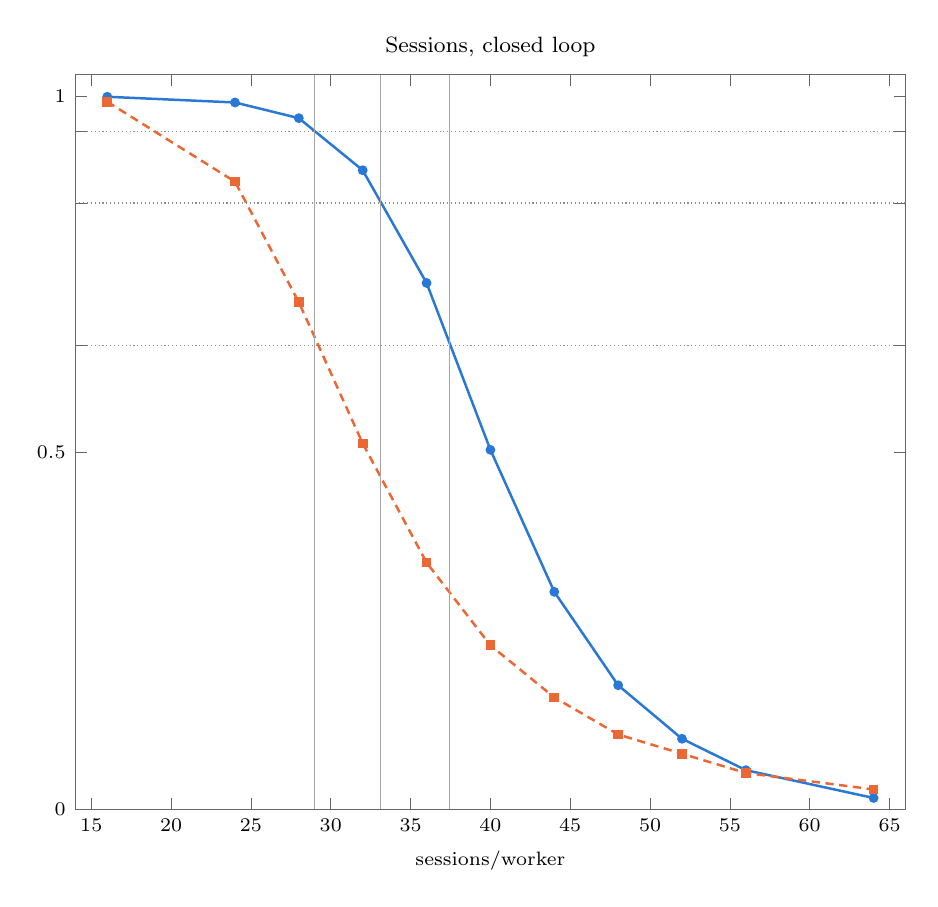
\begin{tikzpicture}
      \begin{axis}[simcurve, title={Sessions, closed loop},
          xlabel={sessions/worker}, xmin=14, xmax=66]
        \addplot[simpi] coordinates {(16,0.999) (24,0.991) (28,0.969) (32,0.896) (36,0.738)
          (40,0.504) (44,0.305) (48,0.174) (52,0.099) (56,0.055) (64,0.016)};
        \addplot[simrr] coordinates {(16,0.992) (24,0.880) (28,0.711) (32,0.513) (36,0.346)
          (40,0.230) (44,0.157) (48,0.105) (52,0.078) (56,0.051) (64,0.028)};
        \simLevelLines{28.9944}{33.1229}{37.4591}
      \end{axis}
    \end{tikzpicture}
  \end{minipage}\hfill
  \begin{minipage}[t]{0.325\linewidth}
    \centering\raisebox{0.45\linewidth}{\pgfplotslegendfromname{simloadlegend}}
  \end{minipage}
  \caption{Calibration load curves at $\Nw = 8$ on train segments: the fraction of in-window
    requests that are good (\cref{eq:good}) under the family's final SLO, for $\piref$
    (blue, solid) and round robin (orange, dashed), averaged over segments and two replicates
    each (6 runs per point for Mooncake and AgentX, 8 for sessions). Dotted horizontal lines
    mark 0.95, 0.85 and 0.65; vertical lines mark the calibrated L1, L2 and L3, where $\piref$'s
    curve crosses them. Top row: each family's primary mode, which also anchors its SLO.}
  \label{fig:load-curves}
\end{figure}

\paragraph{Warm-up and measurement windows.}
% src: CR/facts/calibration.json rules.windows[0..3]; CR/cells/*.jsonl measure (ranges computed
%      2026-10-03: AgentX warmup_ms 1,825,000-13,191,000)
Each cell's measurement window $\win_{\cell}$ (\cref{sec:objective}) starts after a warm-up that
lets caches and queues fill:
\begin{itemize}
  \item \textbf{Open loop, flat traces:} the slice's 4-minute warm-up and 6-minute window (FAST25
    synthetic: 3 minutes and 5.5), divided by the cell's speedup; scored by arrival time.
  \item \textbf{Closed loop:} sessions that arrive during the warm-up are excluded by identity,
    and the window ends at full occupancy, the last instant all sessions are busy; for
    generated sessions, the first twice-the-concurrency sessions are warm-up and the next ten
    times the concurrency are measured.
  \item \textbf{AgentX lanes:} the warm-up is the 90th percentile of the recorded span of the
    cell's plays (\SI{1825}{s} to \SI{13191}{s} of simulated time across cells), and each lane
    gets the fewest copies among 8, 10, 12, 16 and 24 for which its least-loaded lane still
    covers the warm-up plus two mean play spans in every replicate $\krep < 16$.
  \item \textbf{Open loop, generated sessions:} a \SI{540}{s} window after a warm-up long enough
    for the population of open sessions to settle, described next.
\end{itemize}

\paragraph{The session warm-up fix.}
% src: CR/audits/calibration/independent-rerun-r0.md F1 (late window [360, 720]: RR/default 7-43% lower,
%      12/12; 900 s warm-up: s1-n4-L3 default gf 0.814 -> 0.435); CR/facts/calibration.json
%      session_open_warmup.by_transform_tag (fill_at_180s base 0.783, think4.0 0.543)
The first calibration opened the window of open-loop session cells after a fixed \SI{180}{s}
warm-up. An independent re-run of that calibration found that the session population was still
growing then: by a policy-free lifetime model, at \SI{180}{s} it had reached 0.78 of its plateau
at the base think time and 0.54 at four times the think time. The windows therefore mixed a
lightly loaded ramp with saturation. With a \SI{900}{s} warm-up, one train cell labeled L3 had a
$\piref$ good fraction of 0.435 instead of 0.814, and the light ramp had also biased the sessions
knee and so the sessions SLO.
% src: CR/facts/calibration.json rules.windows[1], session_open_warmup (rule_id
%      session-lifetime-p99-kappa3-x2-v1; kappa 3; quantile 99; min_s 180; lifetimes 2;
%      warmup_s 960/1200/1320/2160 by think multiplier), doubled_warmup_check (w1x_vs_w2x
%      gf_default mean_delta -0.00059 se 0.00194, 0/12 |z| > 3; rr_over_default +0.00736;
%      w180_vs_w2x gf_default +0.0606, rr_over_default +0.2167, 12/12 |z| > 3); why_two_lifetimes
The fix sets the warm-up from session lifetimes. A session's envelope lifetime is its summed think
time (scaled by the cell's think multiplier) plus three times its summed uncontended latency
$\Ezero$; the warm-up is twice the 99th percentile of that lifetime over the train sessions,
rounded up to a minute and at least \SI{180}{s}. That gives 960 to \SI{2160}{s}, growing with the
think multiplier. One lifetime (\SI{600}{s} at the base think time) was tried first and failed
the acceptance check. The check replays the same in-window sessions with twice the warm-up
history: across the 12 open-loop session cells that calibration replays (train and validation
cells, plus calibration-only cells on train segments at other $\Nw$), $\piref$'s good
fraction changed by $-0.0006$ on average (standard error 0.0019, no cell beyond three standard
errors) and round robin's goodput ratio to $\piref$ by $+0.0074$, against $+0.061$ and $+0.217$
for the original \SI{180}{s} warm-up on the same sessions.
Per cell, doubling the warm-up history moved $\piref$'s good fraction by up to 0.353 under the
original \SI{180}{s} warm-up (9 of 12 cells beyond 3 standard errors) and by at most 0.014 under
the adopted warm-up of two session lifetimes (no cell beyond 3 standard errors).
% src: CR/facts/calibration.json session_open_warmup.doubled_warmup_check.summary
%      ("w180_vs_w2x|gf_default": max_abs_delta 0.3527, cells_abs_z_gt_3 9 of 12;
%       "w1x_vs_w2x|gf_default": max_abs_delta 0.0142, cells_abs_z_gt_3 0 of 12)
% src: CR/facts/calibration.json sla.synthetic_sessions (knee_rule; outer_fixed_point_history: start
%      within-window drift knee 0.5098, final doubled-history knee 0.45483), fix_r0
%      (sessions_sla_r0 itl 40.4165, slow 1.90627); CR/facts/DEVIATIONS.md 2026-10-03 calibration fixer r0
%      (0.475 and 0.5: gf moved 15-17% when history doubled 1200 s -> 2400 s); STATE.md fix(calibration r0)
With the population settled, the within-window drift test no longer detected the knee: it placed
the sessions knee at 0.510 sessions per second per worker, although at 0.475 and 0.5 doubling the
history still moved $\piref$'s good fraction by 15--17\%. The sessions knee is therefore the load
at which doubling the warm-up history lowers $\piref$'s good fraction by more than 5\%, solved
jointly with the SLO fixed point (0.4548 at $\Nw = 8$). The sessions SLO moved from
$\Imax = \SI{40.4165}{ms}$, $\Smax = 1.90627$ to the values in \cref{tab:calibration}. Only session
cells changed (8 train, 5 validation and 15 test cells); the other families' SLOs, levels and
cells are byte-identical to the first calibration. A second independent re-run then passed.
% src: README "Calibrate, fix r0" (train 8, val 5, test 15); DEVIATIONS (non-session byte-identical
%      train 26/34, val 9/14, test 45/60); STATE.md audit(calibration/independent-rerun r1): PASS

\paragraph{Calibration compute.}
% src: CR/facts/calibration.json summary.calibration_total (13,532 replays, 122,436 replay-s, ~3.3 h
%      local) and fix_r0 (STATE.md: 9,792 replays, 112,561 replay-s)
Calibration took 13,532 replays (about 3.3 hours on one 24-core host), and the session fix
another 9,792.
\Cref{tab:cost} lists it with the rest of the study's compute.

% ---------------------------------------------------------------------------------------------
\subsection{Freeze history}
\label{app:freeze}

% src: CR/facts/test_freeze.json (test_jsonl sha256 7b998b8e..., cells 60; traces: 39 files,
%      2,130,865,265 bytes; trace_sources: 7; cell_content_sha256: 60 entries; engine_json_sha256;
%      split_manifest_sha256; bindings_build_id; rule); CR/cells/SPLIT_MANIFEST.json calibration
%      (cells_version lr-cells-v5)
The freeze record of the frozen cell set holds the SHA-256 of the test cell file
(\code{7b998b8e\ldots}, 60 cells), of each of the 60 test cells' contents, of the 39 trace files
they replay (\SI{2.13}{GB}) and the 7 sources those were derived from, of the engine configuration
and of the split manifest, together with the replay build's identifier. The rule is that nobody
evaluates a test cell before the single test pass, and that pass verifies every hash before it
runs. % prov: lr-cells-v5; "test stage" = the single test pass
% src: CR/facts/test_freeze.json supersedes (b8648ac5..., kept at cells/superseded/calibration-r0/);
%      CR/facts/DEVIATIONS.md 2026-10-03 calibration fixer r0 ("0 test cell ids, test splits or test
%      trace SHAs in 35,735 result records under runs/"); CR/facts/gate.json selection_hygiene
%      (pilot_records_touching_test 0, test_sha_matches_freeze true)
The test set was frozen twice. The first freeze (\code{b8648ac5\ldots}) was replaced after the
session warm-up fix (\cref{app:calibration}); that was allowed because none of the 35,735 result
records then on disk touched a test cell, trace or split. At the end of the pilot, the pilot had
produced no record that touches the test set, and the test file still matched the freeze. The
single test pass verified all 149 freeze hashes before running.
% prov: "pilot gate" = the end of the pilot (the pilot's review)
% src: CR/facts/test_results.json execution.evaluated_once ("149/149 hashes")
